\chapter{Requirements Specification and Project Schedule}

\theoremstyle{plain}
\theoremsymbol{}
\newtheorem{Rule}[theorem]{Rule}

\pagebreak
\section{Requirements Specification} \label{Requirements Specification}
\enlargethispage{2.5cm}
\begin{adjustwidth}{0.23cm}{0cm} \hfuzz=7.0pt
\makebox[\textwidth]{\frame{
\includegraphics[width=17.3cm, page=1]{appendix/Requirements_Specification}}}
\end{adjustwidth}
\newpage

\begin{adjustwidth}{-0.23cm}{0cm} \hfuzz=7.0pt
\makebox[\textwidth]{\frame{
\includegraphics[width=17.3cm, page=2]{appendix/Requirements_Specification}}}
\end{adjustwidth}
\newpage

\begin{adjustwidth}{0.23cm}{0cm} \hfuzz=7.0pt
\makebox[\textwidth]{\frame{
\includegraphics[width=17.3cm, page=3]{appendix/Requirements_Specification}}}
\end{adjustwidth}
\newpage

\begin{adjustwidth}{-0.23cm}{0cm} \hfuzz=7.0pt
\makebox[\textwidth]{\frame{
\includegraphics[width=17.3cm, page=4]{appendix/Requirements_Specification}}}
\end{adjustwidth}
\newpage

\begin{adjustwidth}{0.23cm}{0cm} \hfuzz=7.0pt
\makebox[\textwidth]{\frame{
\includegraphics[width=17.3cm, page=5]{appendix/Requirements_Specification}}}
\end{adjustwidth}
\newpage

\begin{adjustwidth}{-0.23cm}{0cm} \hfuzz=7.0pt
\makebox[\textwidth]{\frame{
\includegraphics[width=17.3cm, page=6]{appendix/Requirements_Specification}}}
\end{adjustwidth}
\newpage

\begin{adjustwidth}{0.23cm}{0cm} \hfuzz=7.0pt
\makebox[\textwidth]{\frame{
\includegraphics[width=17.3cm, page=7]{appendix/Requirements_Specification}}}
\end{adjustwidth}
\newpage


\begin{landscape}
    \section{Project Schedule}
    \begin{figure}[h!]
    	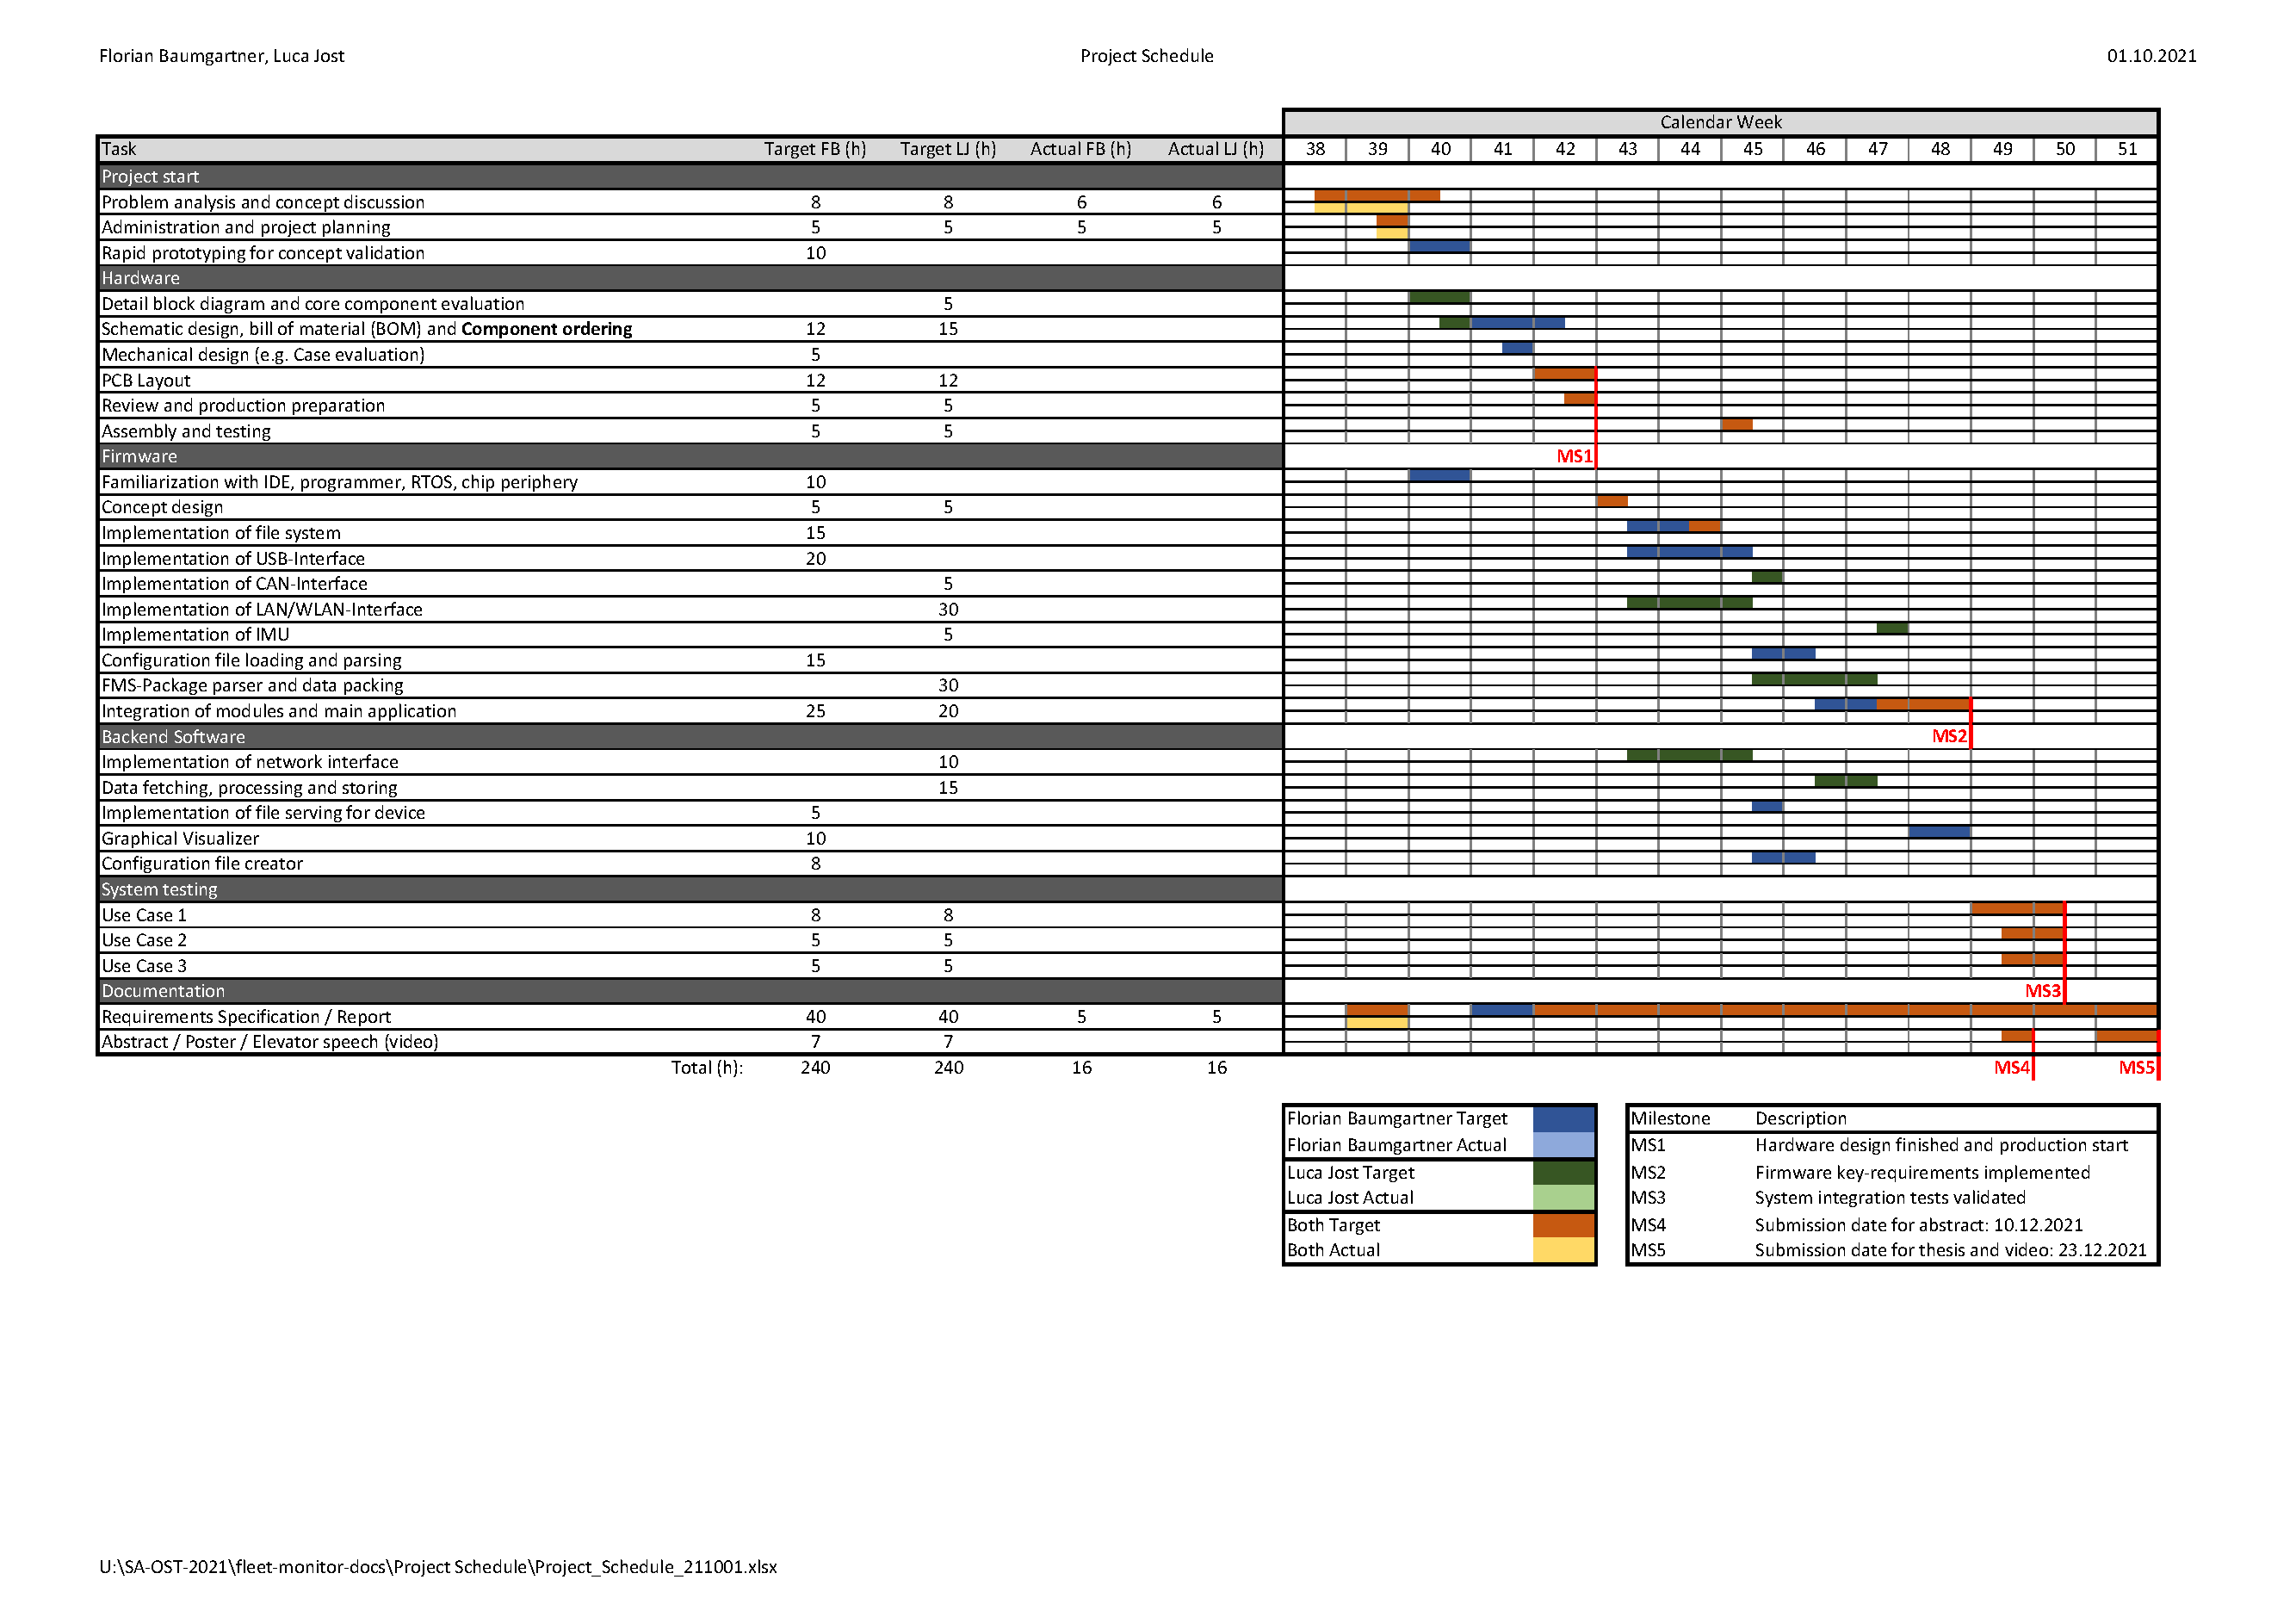
\includegraphics[height=13cm, trim=17mm 69mm 25mm 20mm, clip]{appendix/Project_Schedule_211001}
    	\bigskip
    	\caption{Project Schedule}
	    \vspace{-2cm}
	    \label{fig:project_schedule}
    \end{figure}
    \pagebreak

\end{landscape}